\section{Autonomy Framework}

[MATT/DENIS - 1.5 pg total]

[MATT/JIM] Overview of the Boeing autonomy framework and aircraft used to demonstrate the collision avoidance neural network capability.

Collision avoidance problem -- Strategic rather than tactical, avoidance flight plan must avoid intruder but return to original flight plan

Limitations --  two-dimensional, lateral avoidance maneuvers, focus on single intruder

Describe the safety requirements for collision avoidance.  Maybe reference DO-365. 

Experiments are carried out leveraging the Boeing Autonomy Testbed Aircraft in the form of a Cessna Caravan 208B, tail number N208BX, and is currently serving as a test bed for the DARPA Assured Autonomy program’s air domain (\ref{fig:caravan}).  See Figure X.  The Testbed is optionally piloted and serves as a means to demonstrate commercially viable technologies leading to autonomy.  It is a research and development vehicle able to operate in commercial airspace that is built on open-source middleware with in-house developed guidance and control technologies leveraged from across the Boeing enterprise.  The Testbed includes a full Iron Bird fixture in which new autonomy technology can be fully integrated and tested before flight.  With this Testbed Boeing has demonstrated autonomy firsts including in-air detect and avoid, ADS-B transponder-based route planning for strategic avoidance, and fully autonomous ground taxi.

\begin{figure}
	\centering
	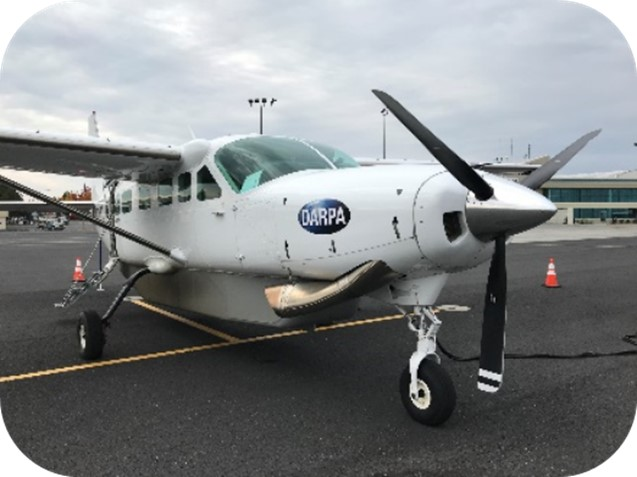
\includegraphics[width=\columnwidth]{figures/caravan.jpg}
	\caption{Boeing Autonomy Testbed Aircraft - Cessna Caravan 208B}
	\label{fig:caravan}
\end{figure}

Detect and avoid mission operating and performance standards are defined in RTCA document DO-365 and includes regulatory guidance for UAS interactions with the National Airspace system, requirement safe operation of aircraft during encounters including separation distance minimums for remaining well clear of aircraft and mid-air collision avoidance, and proper aircraft equipages to achieve safe detect and avoid operations.
The assurance challenged posed herein focuses on the Autonomy Testbed aircraft flying in the vicinity of another intruding airplane, where the Test flight software includes a Boeing-developed LEC to generate an avoidance trajectory for the Testbed to remain well clear of the intruder aircraft as defined in DO-365.  The underlying assurance technology montors the Boeing LEC in order to assess the avoidance trajectory from the LEC.
Figure X shows a detailed view of the autonomy system framework as deployed on the Testbed aircraft.

System elements include: 
\begin{itemize}
\item Perception Sensor – Primary sensor for perceiving the airspace is the Automated Dependent Surveillance Broadcast (ADS-B) providing detection information to the other system functions.
\item ADS-B Tracker – Generates intruder track information from received ADS-B messages to the other system functions.
\item Avoidance Assessment – Evaluates potential future traffic conflicts and issues “alerts” to the Avoidance functions.  Assessment definition and requirements are specified in DO-365 MOPS for DAA System.
\item Baseline (Non AI/ML) Avoidance Guidance – Provides waypoint navigation paths to avoid airspace incursion.  Avoidance computation method is virtual predictive radar which is designed to provide maximum “safe passage timed corridors.”  Avoidance path terminates back on original flight plan.
\item Runtime Assurance Function – SW block representing runtime monitoring and assurance functions concerning LEC and CPS behavior.
\item Autonomous Executive – Constructs and manages execution of the vehicle flight path and contains a SW node to splice in avoidance guidance waypoint paths into the original flight path.
\item Contingency Manager – Maps faults to autonomous actions.  Acts as a deterministic switch between complex functions and recovery actions in reference to ATSM 3269-17 standard.
\item Vehicle Manager – Executes flight path provided by AE including guidance and control for the vehicle.  The VM also sends commands and receives feedback from actuation system components.
\item Actuators / Sensors – Carries out VMS flight control surface commands and provides positional feedback.
\item Ownship State Estimation – Provides vehicle state information including position, altitude, and speed along with the vehicle inertial reference frame.
\item Navigation Database – Reference database of aircraft parameters and airspace waypoints, terrain, airports, approaches, etc.  Used for route/avoidance planning purposes.
\end{itemize}

[DENIS/DRAGOS] Reinforcement learning approach and the LEC produced for collision avoidance.  
Produce avoidance trajectory waypoints  by executing LEC repetitively. 
